\documentclass[]{article}
\usepackage{mathtools}
\usepackage[pdftex]{graphicx}	
\usepackage{amsmath,amsfonts,amsthm}	
\usepackage{tikz}
\usetikzlibrary{chains, positioning}
\newtheorem{theorem}{Theorem}[section]
\newtheorem{lemma}[theorem]{Lemma}
\newtheorem{proposition}[theorem]{Proposition}
\newtheorem{corollary}[theorem]{Corollary}

\theoremstyle{definition}
\newtheorem{definition}{Definition}[section]

\usetikzlibrary{calc,arrows}

%opening
\title{Neural networks are universal approximators}
\author{Rafa\l \vspace{1cm} Skrzypiec}
\date{}
\begin{document}
\maketitle

\begin{center}
	
	
	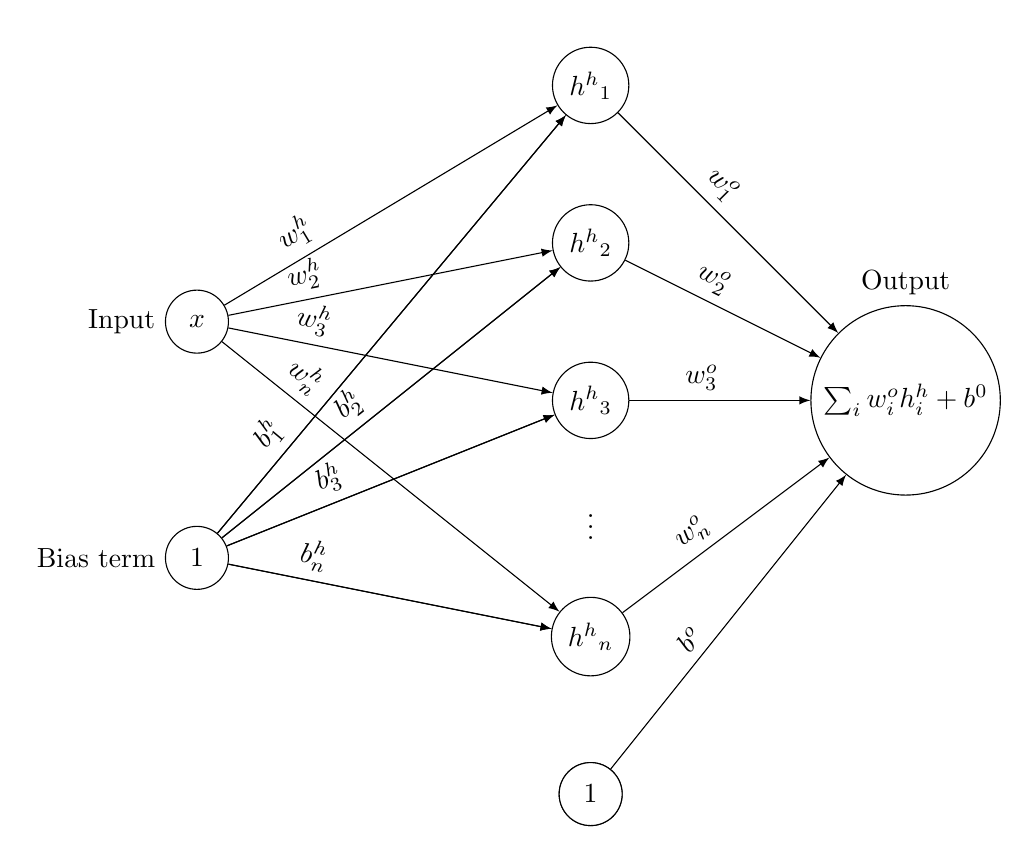
\begin{tikzpicture}
	[   cnode/.style={draw=black,draw=black,fill=#1,minimum width=8mm,circle},
	]
	\tikzset{normal arrow/.style={draw,-latex}}
	\node[cnode=white,label=90:Output] (s) at (9,-6) {$\sum_{i} w^o_{i} h^h_i + b^0$};
	\node[cnode=white,label=180:Bias term] (x-2) at (0,-8) {1};
	\node[cnode=white,label=180:] (p-5) at (5,-11) {1};
	\node at (5,-7.5) {$\vdots$};
	
	\node[cnode=white,label=180:Input] (x-1) at (0,-5) {$x$};
	
	\foreach \x in {1,...,5}
	{
		\pgfmathparse{\x<4 ? \x : "n"}	   
		\ifnum \x = 4
		
		
		\node[cnode=white,label=90:] (p-\x) at (5,{-2.*\x-div(\x,4)}) {${h^h}_n$};
		
		\else
		
		\ifnum \x = 5
		
		
		\node[cnode=white,label=90:] (p-\x) at (5,{-2*\x-div(\x,4)}) {$ 1 $};
		
		\else
		
		\node[cnode=white,label=90:] (p-\x) at (5,{-2*\x-div(\x,4)}) {${h^h}_{\x}$};
		
		\fi
		
		
		\fi
		\ifnum \x = 5
		\path[normal arrow] (p-\x) -- node[above,sloped,pos=0.4] {$b^{o}$} (s);
		\else
		\path[normal arrow] (p-\x) -- node[above,sloped,pos=0.4] {$w^o_{\pgfmathresult}$} (s);
		\fi
	}
	
	
	\foreach \x in {1,...,2}
	{   
		\foreach \y in {1,...,4}
		{   
			\ifnum \x=1
			\ifnum \y=4
			\path[normal arrow] (x-\x) -- (p-\y) node[above,sloped,pos=0.2] {$w^h_{n}$};
			
			\else
			\ifnum \y=5
			\path[normal arrow] (x-\x) -- (p-\y) node[below,sloped,pos=0.15] {$w_{w n+1}$};
			\else 
			\path[normal arrow] (x-\x) -- (p-\y) node[above,sloped,pos=0.25] {$w^h_{\y}$};
			
			\fi
			\fi
			\else
			\path[normal arrow] (x-\x) -- (p-\y); 		
			\fi
			
			\ifnum \x=2
				\ifnum \y=4
				\path[normal arrow] (x-\x) -- (p-\y) node[above,sloped,pos=0.25] {$b^h_{n}$};
					\else
				\ifnum \y=2
				\path[normal arrow] (x-\x) -- (p-\y) node[above,sloped,pos=0.42] {$b^h_{\y}$};
					\else
				\ifnum \y=3
								\path[normal arrow] (x-\x) -- (p-\y) node[above,sloped,pos=0.34] {$b^h_{\y}$};
				
				\else
				
					\path[normal arrow] (x-\x) -- (p-\y) node[above,sloped,pos=0.2] {$b^h_{\y}$};
					\fi
					\fi
				\fi
			\fi
			%\draw (x-\x) -- (p-\y) node[above,sloped,pos=0.3] {$\omega_{\x\y}$};
		}
	}
	\end{tikzpicture}
	
\end{center}


\newpage
\section{Universal approximation theorem}

Universal approximation theorem states that a feedforward neural network with one hidden layer and finite but sufficiently large number of neurons can approximate to arbitrary accuracy any functional continuous mapping from one finite-dimensional space to another. 


The theorem was proved by Hornik, Stinchcombe and White in 1989 [cytowanie], but before that paper was published, in the same year, Cybenko [cytowanie] had proved universal approximation property for feedforward neural network using sigmoidal activation functions.

Sigmoidal functions is family of functions widely used in Feedforward neural networks, especially for regression purposes.

In this section, I present a proof given by Cybenko in 1989, then I will demonstrate a visual proof of universal approximation theorem using sigmoidal activation functions.



\subsection{Approximation by Superpositions of a Sigmoidal Functions}

Let $I_n$ denotes the $n$-dimensional unit cube, $[0,1]^n$. $C(I_n)$ refers to the space of continous functions on $I_n$. In addition, let $M(I_n)$ denotes space of finite, signed regular Borel measures on $n$-dimensional unit cube $I_n$. 


\begin{definition}
Measure $\mu$ is regural if for every measurable set $A$, $\mu(A)$ equals the supremum of the measures of closed subsets of $A$ and the infimum of open supersets of $A$. [Probability measures on metric spaces K.R. Parthasarathy]	
\end{definition}
 
 
%\begin{definition} Zobaczymy czy się przyda
%	$f:I_n \rightarrow C(I_n),$
%	$||f|| = \sup {|f(x)| : x \in I_n }$.
%\end{definition}
% 
% 
% $||f||$ is used to denote the supremum norm of an $f \in C(I_n)$. 

\begin{definition}
	It is said that $\sigma: \mathbb{R} \rightarrow \mathbb{R}$ is sigmoidal if
	\begin{eqnarray*}
		\sigma(x) \rightarrow \begin{cases} 1 \;\;\;\text{as} &x \rightarrow +\infty\\ 0 \;\;\;\text{as} &x \rightarrow -\infty\end{cases}
	\end{eqnarray*}
	
\end{definition}



\begin{definition}
It is said that $\sigma$ is discriminatory if for a measure $\mu \in M(I_n)$ 

\begin{equation}
\int_{I_n} \sigma \left( w^\mathsf{T}x + b_0 \right) d\mu(x) = 0
\end{equation}
for all $w\in \mathbb{R}$ and $b_0 \in \mathbb{R}$ implies that $\mu = 0$.
	
\end{definition}


\begin{theorem}
Any bounded, measurable sigmoidal function, $\sigma$, is discriminatory. In particular, any continuous sigmoidal function is discriminatory.
[cytowanie Cybenko]
\end{theorem}


Proof of Cybenko's theorem requires to introduce more useful definitions and theorems. Hahn-Banach theorem is a general theorem which says that any functional can be extended to the whole space while retaining the desired properties.


\begin{theorem}[Hahn-Banach theorem]
	
	
	Let $X$ be a real vector space, $p$ a real-valued function defined on $X$ satisfying 
	
	$$	p \left(\alpha x + (1-\alpha) y \right) \leq \alpha p(x)  + (1 - \alpha)p(y) \;\;\;\;\;\; \forall \alpha \in \left[0,1\right], x, y \in X$$
	
	Suppose that $\lambda$ is a linear functional defined on a subspace $Y\subset X $ which satisfies 
	$$\lambda(x) \leq p(x) \;\;\;\;\;\; \forall x \in Y.$$
	
	Then, there is a linear functional $\Lambda$, defined on $X$, satisfying 
	$$\Lambda(x) \leq p(x) \;\;\;\;\;\; \forall x \in X,$$
	
	such that $$\Lambda(x) = \lambda(x) \;\;\;\;\;\; \forall x \in Y.$$
	

Reed \& Simon (1980), Methods of Modern Mathematical Physics. Functional Analysis
\end{theorem}


\begin{definition}	
	The space $\mathcal{L}\left(\mathcal{H}, \mathbb{C}\right)$ is called the dual space of Hilbert space $\mathcal{H}$ and is denoted by $\mathcal{H^*}$. The elements of $\mathcal{H^*}$ are called continuous linear functionals. 
	
Reed \& Simon (1980), Methods of Modern Mathematical Physics. Functional Analysis
	
\end{definition}	

The following important theorem characterizes $\mathcal{H^*}$ and it was formulated by F. Riesz.

	
\begin{theorem}[Riesz Representation Theorem]
	
	For each $T \in \mathcal{H^*}$, there is a unique $y_T \in \mathcal{H}$ such that $$T(x) = \langle y_T, x \rangle \;\;\;\;\;\; \forall x \in \mathcal{H} $$
	
	
In addition $$||y_T ||_{\mathcal{H}}  = ||T||_{\mathcal{H^*}}$$

Reed \& Simon (1980), Methods of Modern Mathematical Physics. Functional Analysis

\end{theorem}


\begin{theorem}[]
	Let $\sigma$ be any continous discriminatory function. Then finite sums of the form
\begin{equation}
G\left(x\right) = \sum_{i=1}^{N} w^{o}_i \sigma\left({w^h_i}^{\mathsf{T}}x + b^h_i\right)
\end{equation}


are dense in $C(I_n)$. In other words, given any $f \in C(I_n)$ and $\epsilon >0$, there is a sum, $G(x)$, of the above form, for which

$$
|G(x) - f(x)| < \epsilon \;\;\;\;\;\;\;\; \forall x \in I_n
$$
\end{theorem}

\begin{proof}

Let $S \subset C(I_n)$ be the set of functions of the form $G(x)$ or in other words - set of neural networks. Clearly $S$ is a linear subspace of $C(I_n)$. If $S$ is dense, the closure of $S$ is all of $C(I_n)$. 


Assume that closure of $S$ is not all of $C(I_n)$. Then the closure of $S$, say $S'$, is a closed proper subspace of $C(I_n)$. By the Hahn-Banach Theorem, there exists a bounded linear functional on $C(I_n)$, call it L, with the property that $L \neq 0$ but $L(S') = L(S) = 0$.

By the Riesz Representation Theorem, this bounded linear functional, L, is of the following form 

$$
L(h) = \int_{I_n} h(x)d\mu(x)
$$

for some $\mu \in M(I_n)$, for all $h \in C(I_n)$. In particular, since $\sigma(w^\mathsf{T}x + b)$ is in $S'$ for all $w$ and $b$, we must have that

$$
\int_{I_n} \sigma \left(w^\mathsf{T}x + b \right) d\mu(x) = 0 
$$

However, we assumed that $\sigma$ was discriminatory so that this condition implies that $\mu = 0$ contradicting our assumption. Hence, the subspace $S$ must be dense in $C(I_n)$.

This demonstrates that sums of the form

$$
G\left(x\right) = \sum_{i=1}^{N} w^{o}_i \sigma\left({w^h_i}^{\mathsf{T}}x + b^h_i\right)
$$

are dense in $C(I_n)$ providing that $\sigma$ is continuous and discriminatory.

\end{proof}

\newpage

\section{Visual representation}

\begin{figure}[h!]
	\centering
	\includegraphics[width=\linewidth]{cybenko14_12_1}

\end{figure}

\begin{figure}[h!]
	\centering
	\includegraphics[width=\linewidth]{mse}

\end{figure}




%\begin{table}
%		\begin{center}
%	\begin{tabular}{ | l | c | }
%		\hline
%		Number of hidden neurons & Mean squared error \\ \hline
%		1 & 0.00942516615858  \\ \hline
%		2 & 0.00277472585580  \\ \hline
%		3 & 0.00135999931016  \\ \hline
%		4 & 5.33546419190e-05  \\ \hline
%		10 & 1.70243920789e-06  \\ \hline
%		100 & 1.11243069317e-06  \\ \hline
%		\hline
%	\end{tabular}
%		\end{center}
%\end{table}



\newpage
\subsection{Data}

The training set has $m$ samples of $1$ dimension, it is given as a vector: $X \in \mathbb{R}^{1\times m}$ and corresponding results
$Y\in \mathbb{R}^{1\times m}$.

\subsection{Parameters}

The net will have 2 layers: 1) a hidden one, having $L$ neurons,
and 2) an output one, having $1$ neuron.

The layers are defined through:

1. the parameters of the hidden layer, which maps $1$-dimensional input vectors
into activations of $L$ neurons:
weight matrix $W^h\in\mathbb{R}^{L\times 1	}$ and bias vector
$b^h\in\mathbb{R}^{L\times 1}$,

2. the parameters of the output layer, which maps $L$-dimensional vector
of activations of the hidden layer to 1 activations of output neurons:
weight matrix $W^o\in{1\times L}$ and bias vector $b^o\in\mathbb{R}^{1\times 1}$.


\subsection{Signal forward propagation (fprop)}

Each hidden neuron computes its total input as a sum of product of its
inputs, weight matrix and bias. For an $i$-th sample,
the total input
${a^{h}}^{(i)}_l $ of an $I$-th neuron is thus:
\begin{equation}
{a^h}^{(i)}_l = {W^h}_{l}x^{(i)} + {b^h}_l
\end{equation}
The total input of neurons might also be expressed via matrices,
using matrix multiplication and broadcasting (which allows to add
a column vector to all column vectors of a matrix):
\begin{equation}
{a^h} = W^h\cdot x + b^h
\end{equation}
This can be implemented in Python as $ah = W.dot(x) + b$

Next, we compute activation $h^h$ of hidden neurons with sigmoid
$\sigma(a) = \frac{1}{1+e^{-a}}$:
\begin{equation}
{h^h}^{(i)}_l=\sigma({a^h}^{(i)}_l)
\end{equation}
Thanks to vectorization in Python + numpy, $h^h$ might be computed with a single
expression $hh = numpy.sigmoid(ah)$.

Finally, total input of the output layer can be computed using
activations of the hidden layer (with the help of broadcasting) as:


\begin{equation}
a^o = W^o\cdot h^h + b^o
\end{equation}

And for I-th sample we have:

\begin{equation}
\begin{split}
{a^o}^{(i)} &= {W^o}_l{h^h}^{(i)}_l + {b^o} \\
& = {W^o}_l\sigma({a^h}^{(i)}_l) + {b^o} \\
& = {W^o}_l\sigma({W^h}_{l}x^{(i)} + {b^h}_l) + {b^o}
\end{split}
\end{equation}




We will use mean squared error as the loss function:

\begin{equation}
\begin{split}
J^{(i)}(\Theta) &= \frac{1}{2} \left( y^{(i)}- a^{o{(i)}}  \right)  ^2 \\
J(\Theta) &= \frac{1}{m}\sum_{i=1}^m J^{(i)}(\Theta)= \frac{1}{2m}\sum_{i=1}^m \left( y^{(i)}- a^{o{(i)}}  \right)  ^2  .
\end{split}
\end{equation}


\subsection{Error backpropagation (bprop)}

Using the chain rule one can derive the gradient of the loss function
in respect to neurons' activations and network parameters.


First we compute the gradient with respect to the output layer's
total inputs:

\begin{equation}
\frac{\partial J}{\partial {a^o}^{(i)}} = \frac{1}{m} \left( y^{(i)}- a^{o{(i)}}  \right),
\end{equation}

then we compute the gradient with respect to activations of hidden units:

\begin{equation}
\frac{\partial J}{\partial {h^h}^{(i)}_l} = \frac{\partial J}{\partial {a^o}^{(i)}} \frac{\partial {a^o}^{(i)}}{\partial {h^h}^{(i)}_l} =  \frac{\partial J}{\partial {a^o}^{(i)}} {W^o}_{l},
\end{equation}
then we compute the gradient with respect to the total activations of hidden units:

\begin{equation}
\frac{\partial J}{\partial {a^h}^{(i)}_l} = \frac{\partial J}{\partial {h^h}^{(i)}_l}\frac{\partial {h^h}^{(i)}_l}{\partial {a^h}^{(i)}_l} = \frac{\partial J}{\partial {h^h}^{(i)}_l} {h^h}^{(i)}_l(1-{h^h}^{(i)}_l) 
\end{equation}

where we have used the relationship
$$\frac{\partial \sigma(x)}{\partial x} = \sigma(x)(1-\sigma(x))$$	.


Finally we can use the gradients with respect to the total inputs to
compute the gradients with respect to network parameters,
eg. for the input layer:

\begin{equation}
\frac{\partial J}{\partial {W^o}_{l}} = \sum_{i}\frac{\partial J}{\partial {a^o}^{(i)}}\frac{\partial {a^o}^{(i)}}{\partial {W^o}_{l}} = \sum_{i}\frac{\partial J}{\partial {a^o}^{(i)}}{h^h}^{(i)}_l,
\end{equation}

\begin{equation}
\frac{\partial J}{\partial {b^o}} = \sum_{i}\frac{\partial J}{\partial {a^o}^{(i)}}\frac{\partial {a^o}^{(i)}}{\partial {b^o}} = \sum_{i}\frac{\partial J}{\partial {a^o}^{(i)}}.
\end{equation}



\end{document}





wiki: "A sigmoid function is a mathematical function having a characteristic "S"-shaped curve or sigmoid curve. Often, sigmoid function refers to the special case of the logistic function defined by the formula"

$$
\sigma(x) = \frac{1}{1+e^{-x}}
$$





\begin{center}
	
	
	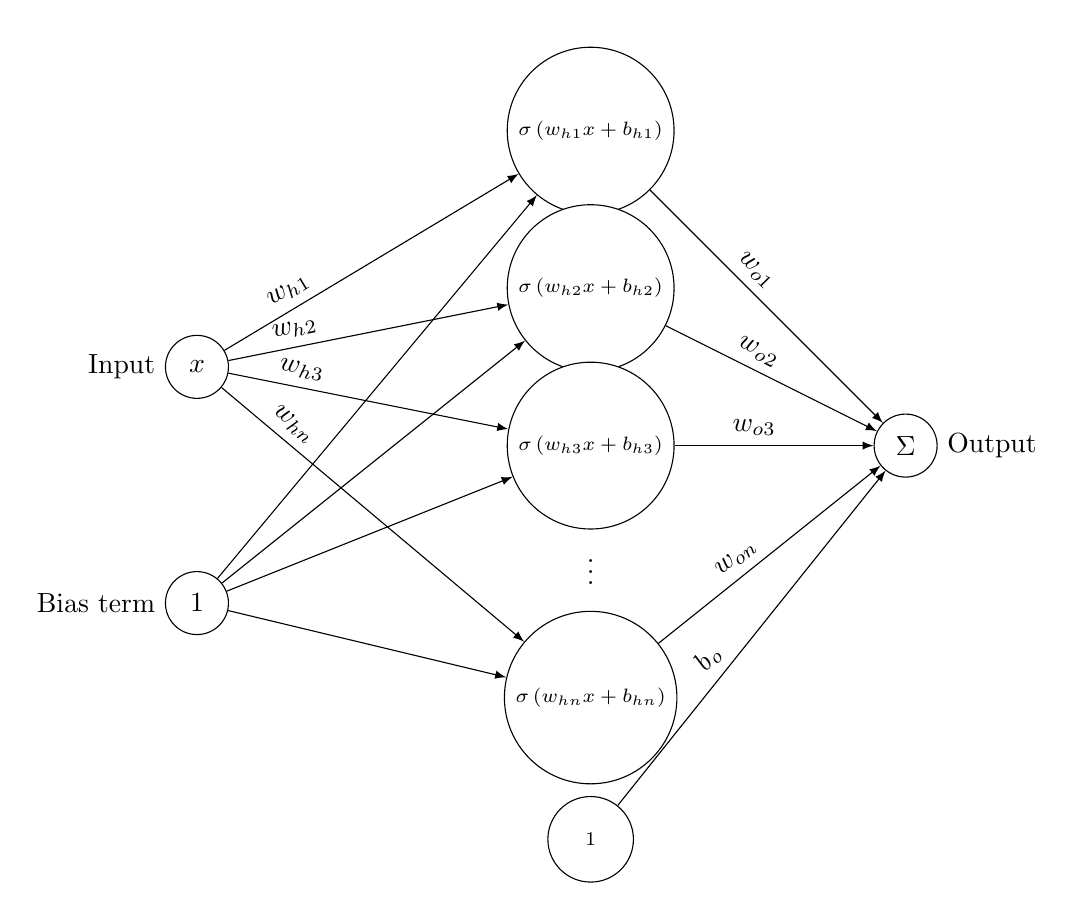
\begin{tikzpicture}
	[   cnode/.style={draw=black,draw=black,fill=#1,minimum width=8mm,circle},
	]
	\tikzset{normal arrow/.style={draw,-latex}}
	\node[cnode=white,label=0:Output] (s) at (9,-6) {$\Sigma$};
	\node[cnode=white,label=180:Bias term] (x-2) at (0,-8) {1};
	\node[cnode=white,label=180:] (p-5) at (5,-11) {1};
	\node at (5,-7.5) {$\vdots$};
	
	\node[cnode=white,label=180:Input] (x-1) at (0,-5) {$x$};
	
	\foreach \x in {1,...,5}
	{
		\pgfmathparse{\x<4 ? \x : "n"}	   
		\ifnum \x = 4
		
		
		\node[cnode=white,label=90:] (p-\x) at (5,{-2.05*\x-div(\x,4)}) {\scriptsize$\sigma\left(w_{hn}x + b_{hn}\right)$};
		
		\else
		
		\ifnum \x = 5
		
		
		\node[cnode=white,label=90:] (p-\x) at (5,{-2*\x-div(\x,4)}) {\scriptsize$\;\;\; \; 1 \; \;\;\;$};
		
		\else
		
		\node[cnode=white,label=90:] (p-\x) at (5,{-2*\x-div(\x,4)}) {\scriptsize$\sigma\left(w_{h\x}x + b_{h\x}\right)$};
		
		\fi
		
		
		\fi
		\ifnum \x = 5
		\path[normal arrow] (p-\x) -- node[above,sloped,pos=0.4] {$b_{o}$} (s);
		\else
		\path[normal arrow] (p-\x) -- node[above,sloped,pos=0.4] {$w_{o\pgfmathresult}$} (s);
		\fi
	}
	
	
	\foreach \x in {1,...,2}
	{   
		\foreach \y in {1,...,4}
		{   
			\ifnum \x=1
			\ifnum \y=4
			\path[normal arrow] (x-\x) -- (p-\y) node[above,sloped,pos=0.2] {$w_{h n}$};
			
			
			\else
			\ifnum \y=5
			\path[normal arrow] (x-\x) -- (p-\y) node[below,sloped,pos=0.15] {$w_{w n+1}$};
			\else 
			\path[normal arrow] (x-\x) -- (p-\y) node[above,sloped,pos=0.25] {$w_{h\y}$};
			
			\fi
			\fi
			\else
			\path[normal arrow] (x-\x) -- (p-\y); 
			
			\fi
			
			%\draw (x-\x) -- (p-\y) node[above,sloped,pos=0.3] {$\omega_{\x\y}$};
		}
	}
	\end{tikzpicture}
	
\end{center}



\def\layersep{2.5cm}
\begin{center}
	
	
	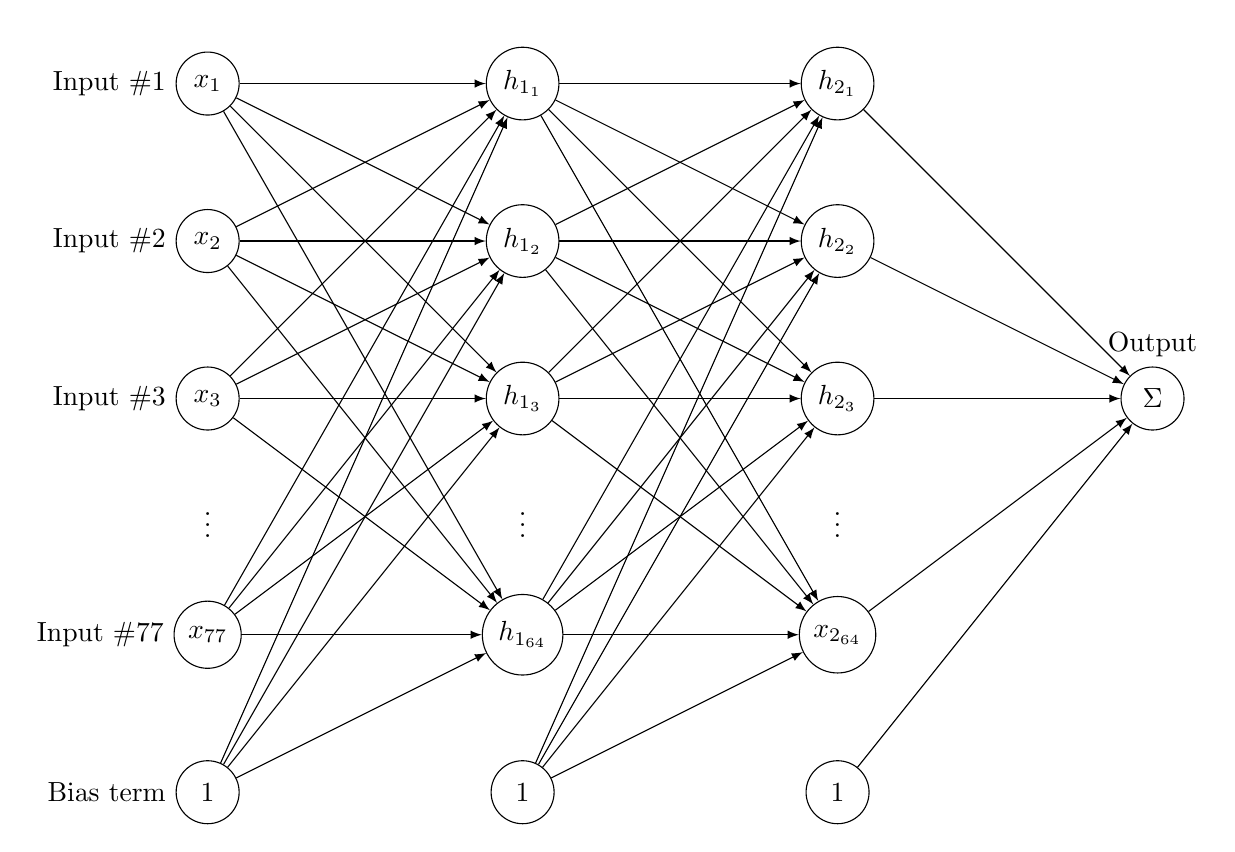
\begin{tikzpicture}
	[   cnode/.style={draw=black,draw=black,fill=#1,minimum width=8mm,circle},
	]
	\tikzset{normal arrow/.style={draw,-latex}}
	\node[cnode=white,label=90:Output] (s) at (12,-6) {$\Sigma$};
	\node at (0,-7.5) {$\vdots$};
	
	\node[cnode=white,label=180:Bias term] (x-5) at (0,-11) {1};
	
	\node at (4,-7.5) {$\vdots$};
	
	\node at (8,-7.5) {$\vdots$};
	
	\node[cnode=white,label=180:] (p-5) at (4,-11) {$1$};
	
	\node[cnode=white,label=180:] (z-5) at (8,-11) {$1$};
	
	
	\foreach \x in {1,...,4}
	{
		\pgfmathparse{\x<4 ? \x : "n"}	   
		\ifnum \x = 4
		\node[cnode=white,label=180:Input \#77] (x-\x) at (0,{-2*\x-div(\x,4)}) {$x_{77}$};
		\node[cnode=white,label=90:] (p-\x) at (4,{-2*\x-div(\x,4)}) {$h_{1_{64}}$};
		
		\node[cnode=white,label=90:] (z-\x) at (8,{-2*\x-div(\x,4)}) {$x_{2_{64}}$};
		
		\else
		
		\node[cnode=white,label=180:Input \#\pgfmathresult] (x-\x) at (0,{-2*\x-div(\x,4)}) {$x_{\x}$};
		\node[cnode=white,label=90:] (p-\x) at (4,{-2*\x-div(\x,4)}) {$h_{1_{\x}}$};
		
		\node[cnode=white,label=90:] (z-\x) at (8,{-2*\x-div(\x,4)}) {$h_{2_{\x}}$};
		
		\fi
		\path[normal arrow] (z-\x) -- node[above,sloped,pos=0.4] {} (s);
	}
	
	
	\foreach \x in {1,...,5}
	{   
		\foreach \y in {1,...,4}
		{   
			\ifnum \x=1
			\ifnum \y=4
			\path[normal arrow] (x-\x) -- (p-\y) node[above,sloped,pos=0.15] {};
			
			\else
			\path[normal arrow] (x-\x) -- (p-\y) node[above,sloped,pos=0.2] {};
			\fi
			\else
			\path[normal arrow] (x-\x) -- (p-\y); 
			
			\fi
			
			
			\ifnum \x=1
			\ifnum \y=4
			\path[normal arrow] (p-\x) -- (z-\y) node[above,sloped,pos=0.15] {};
			
			\else
			\path[normal arrow] (p-\x) -- (z-\y) node[above,sloped,pos=0.2] {};
			\fi
			\else
			\path[normal arrow] (p-\x) -- (z-\y); 
			
			\fi
			
			
			
			%\draw (x-\x) -- (p-\y) node[above,sloped,pos=0.3] {$\omega_{\x\y}$};
		}
		
		
		
		\ifnum \x=5
		\path[normal arrow] (z-\x) -- node[above,sloped,pos=0.4] {} (s);
		\else
		
		\fi
	}
	\end{tikzpicture}
	
\end{center}

